\documentclass{article}
\usepackage{enumerate}
\usepackage{amsmath}
\usepackage{amssymb}
\usepackage{graphicx}
\usepackage{subfigure}
\usepackage{geometry}
\usepackage{caption}
\usepackage{indentfirst}
\usepackage{array}
%\renewcommand\arraystretch{2}
\usepackage{tikz}
\usepackage{multicol}
\usepackage{algorithm}  
\usepackage{algorithmicx}  
\usepackage{algpseudocode}
\renewcommand{\algorithmicrequire}{\textbf{Input:}}  
\renewcommand{\algorithmicensure}{\textbf{Output:}}  
\usepackage{minted}
\usemintedstyle{autumn}
\geometry{left=3.0cm,right=3.0cm,top=3.0cm,bottom=4.0cm}
\renewcommand{\thesection}{Ex. \arabic{section}}
\title{VE281 Writing Assignment Four}
\author{Liu Yihao 515370910207}
\date{}

\begin{document}
\maketitle

\section{}
\begin{enumerate}[(a)]
\item\ 
\begin{center}
\begin{tikzpicture}
\tikzstyle{every node}=[draw,shape=circle,minimum size=0.8cm];
\node {4}[sibling distance=4cm]
child { node {2}[sibling distance=2cm]
	child {
		node {1}[sibling distance=1cm]
	}
	child {
		node {3}[sibling distance=1cm]
	}
}
child { node {9}[sibling distance=2cm]
	child[left] {
		node {5}[sibling distance=1cm]
		child[right] { 
			node {7}[sibling distance=1cm]
			child[left] { node {6} }
			child[right] { node {8} }
		}
	}
};
\end{tikzpicture}
\end{center}
\item\ 
\begin{center}
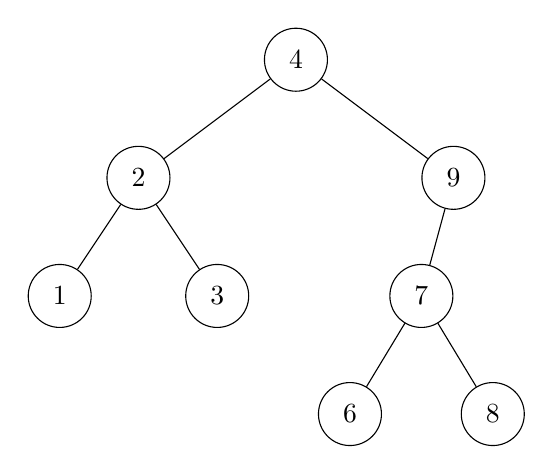
\begin{tikzpicture}
\tikzstyle{every node}=[draw,shape=circle,minimum size=0.8cm];
\node {4}[sibling distance=4cm]
child { node {2}[sibling distance=2cm]
	child {
		node {1}[sibling distance=1cm]
	}
	child {
		node {3}[sibling distance=1cm]
	}
}
child { node {9}[sibling distance=2cm]
	child[left] {
		node {7}[sibling distance=1cm]
		child[left] { node {6} }
		child[right] { node {8} }
	}
};
\end{tikzpicture}
\end{center}
\item\ 
\begin{center}
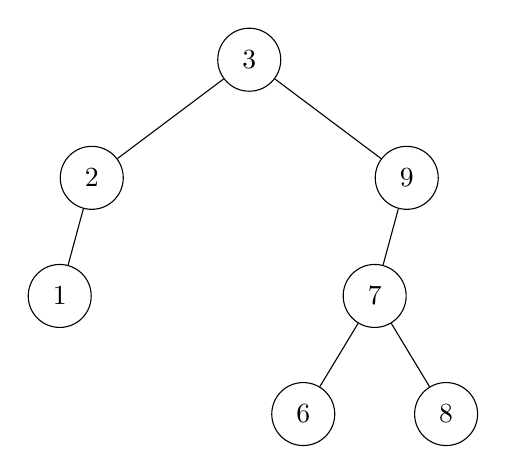
\begin{tikzpicture}
\tikzstyle{every node}=[draw,shape=circle,minimum size=0.8cm];
\node {3}[sibling distance=4cm]
child { node {2}[sibling distance=2cm]
	child[left] {
		node {1}[sibling distance=1cm]
	}
}
child { node {9}[sibling distance=2cm]
	child[left] {
		node {7}[sibling distance=1cm]
		child[left] { node {6} }
		child[right] { node {8} }
	}
};
\end{tikzpicture}
\end{center}
\end{enumerate}

\section{}
\begin{algorithm}[H]
    \begin{algorithmic}
        \Require A non-empty binary tree with root node $root$
        \Ensure Whether the tree is a binary search tree
        \Function{examine}{$root$}
            \If {$root.left$ is empty}
                \State $flag\gets true$
            \ElsIf {$root.left.key>root.key$}
                \State $flag\gets false$
            \Else
                \State $flag\gets$ \Call{examine}{$root.left$}
            \EndIf
            \If {\textbf{not} $flag$}
                \State \Return {flag}
            \EndIf
            \If {$root.right$ is empty}
                \State $flag\gets true$
            \ElsIf {$root.right.key<root.key$}
                \State $flag\gets false$
            \Else
                \State $flag\gets$ \Call{examine}{$root.right$}
            \EndIf
            \State \Return $flag$
        \EndFunction
    \end{algorithmic}  
\end{algorithm}

We know that if we want to ensure the tree is a binary search tree, at least every node should be verified once. In my algorithm, each node is verified exactly once, which should be a most runtime-efficient one. The runtime is $\Theta(n)$.

\section{}
\begin{minted}{c++}
node* getPredHelper(node* root, Key key, node* parent) {
    if (root == NULL) return NULL;
    if (root->key == key) {
        if (root->left) return findMax(root->left);
        return root;
    }
    node *temp = NULL;
    if (root->key < key) temp = getPredHelper(root->left, key, root);
    if (!temp) temp = getPredHelper(root->right, key, root);
    if (!temp) return NULL;
    if (temp->key == key) {
        if (!parent) return NULL;
        if (root->key < key) return root;
    }
    return temp;
}

node* getPred(node* root, Key key) {
    return getPredHelper(root, key, NULL);
}
\end{minted}

\section{}
\begin{center}
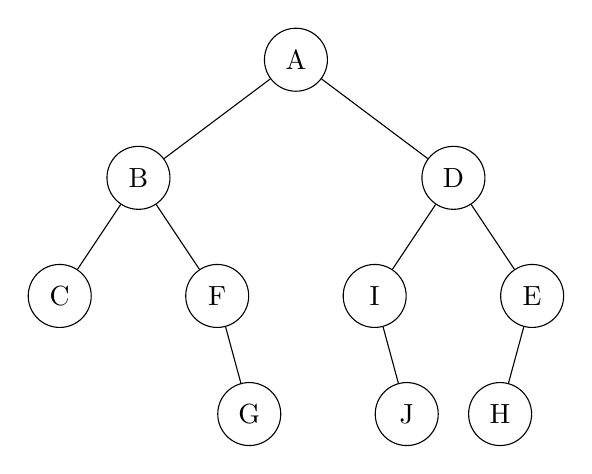
\begin{tikzpicture}
\tikzstyle{every node}=[draw,shape=circle,minimum size=0.8cm];
\node {A}[sibling distance=4cm]
child { node {B}[sibling distance=2cm]
	child {
		node {C}[sibling distance=1cm]
	}
	child {
		node {F}[sibling distance=1cm]
		child[right] { 
			node {G}[sibling distance=1cm]
		}
	}
}
child { node {D}[sibling distance=2cm]
	child {
		node {I}[sibling distance=1cm]
		child[right] { 
			node {J}[sibling distance=1cm]		
		}
	}
	child {
		node {E}[sibling distance=1cm]
		child[left] { 
			node {H}[sibling distance=1cm]
		}
	}
};
\end{tikzpicture}
\end{center}

\end{document}
